\section*{Лекція 4: Списки}
\subsection{Списки та операції над ними} 
\begin{frame}
\frametitle{Створення списків у Python}
Список - впорядкована колекція даних різних типів.

Список відноситься до змінних типів даних.

Пустий список - []. Для створення списку на основі об'єкту, який можна перебирати, використовується функція list.
\begin{figure}
\begin{center}
 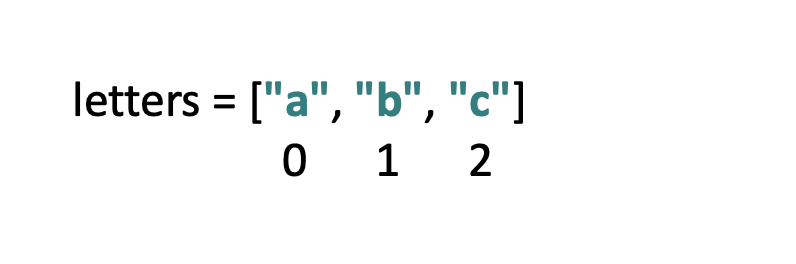
\includegraphics[width=0.6\textwidth]{pictures/list.png}
\caption{Список}
\label{list} 
\end{center}
\end{figure}

\end{frame}

 
\begin{frame}
\frametitle{Основні  функції для роботи зі списком s}
    \begin{itemize}
        \item<1-> \texttt{len(s)} - визначення числа елементів у списку;
        \item<2-> \texttt{max(s)} - знаходження максимального значення;
        \item<2-> \texttt{min(s)} - знаходження мінімального значення;
        \item<3-> \texttt{sum(s)} - розрахунок суми;
        \item<4-> \texttt{sorted(s)} - сортування за зростанням;
        \item<4-> \texttt{sorted(s, reverse=True)} - сортування за спаданням.
    \end{itemize}
\end{frame}

\begin{frame}
\frametitle{Оператори для роботи зі списками}
    \begin{itemize}
        \item<1-> \texttt{+} - поєднання двох списків в один;
        \item<2-> \texttt{*} - повторення списку;
        \item<3-> \texttt{in} - перевірка входження елементу в список;
        \item<4-> \texttt{del} - видалення елементу списку.
    \end{itemize}
\end{frame}

\subsection{Робота зі списками} 
\begin{frame}
\frametitle{Зрізи}
Зрізи дозволяють отримати деяку підмножину значень списку:
\vspace{1cm}
\begin{center}
\huge{lst[start:stop[:step]]}
\end{center}
\normalsize

\end{frame}


\begin{frame}
\frametitle{Копіювання та порівнювання списків}
Для створення копії списка \texttt{lst} використовується команда \texttt{lst[:]} або \texttt{list(lst)}.

Списки можна лексикографічно порівнювати між собою за допомогою операторів: >, <, == та !=.
\begin{table}
  \caption{}
  \label{tab:}

  \begin{center}
    \begin{tabular}{|c|c|}
    \hline
      \textbf{Оператор} & \textbf{Значення} \\
      \hline
      > & більше \\
      \hline
      < & менше\\
      \hline
      == & дорівнює \\
      \hline
      != & не дорівнює\\
      \hline
    \end{tabular}
  \end{center}
\end{table}
\end{frame}

\subsection{Методи списків} 

\begin{frame}
\frametitle{Додаванна та видалення елементів}
\begin{center}
\texttt{об'єкт.метод(аргументи)}
\end{center}
\begin{itemize}
        \item<1-> \texttt{lst.append(el)} - додати елемент el в кінець списку lst;
        \item<2-> \texttt{lst.insert(pos, el)} - додати елемент el до списку lst на місце з індексом pos;
        \item<3-> \texttt{lst.remove(val)} - видаляє перший елемент val зі списку lst (якщо елементу немає в списку, отримуємо помилку);
        \item<4-> \texttt{lst.pop([ind])} - видаляє та \textbf{повертає} останній елемент зі списку lst або елемент з індексом ind.
    \end{itemize}
\end{frame}


\begin{frame}
\frametitle{Аналіз списку}
\begin{center}
об'єкт.метод(аргументи)
\end{center}
\begin{itemize}
        \item<1-> \texttt{lst.clear()} - видаляє всі елементи зі списку lst;
        \item<2-> \texttt{lst.copy()} - повертає копію списку lst;
        \item<3-> \texttt{lst.count(val)} - число елементів зі значенням val в списку lst;
        \item<4-> \texttt{lst.index(val)} - індекс значення val в списку lst;
        \item<4-> \texttt{lst.index(val, start)} - знаходить індекс значення val в списку lst, починаючи з індексу start;
    \end{itemize}
\end{frame}

\begin{frame}
\frametitle{Зміна списку}
\begin{center}
об'єкт.метод(аргументи)
\end{center}
\begin{itemize}
        \item<1-> \texttt{lst.reverse()} - змінює порядок елементів списку lst на зворотній;
        \item<2-> \texttt{lst.sort()} - сортує елементи списку lst за зростанням;
        \item<2-> \texttt{lst.sort(reverse=True)} - сортує елементи списку lst за спаданням;
    \end{itemize}
\end{frame}

\subsection{Додаткові відомості щодо списків} 

\begin{frame}
\frametitle{Вкладені списки} 
\begin{center}
Вкладений список це двовимірний список.

\vspace{1cm}

\Large
lst = [line[:], line[:], line[:]]
\normalsize

\vspace{1cm}

Щоб отримати один елемент використовуємо команду lst[i][j]. 
\end{center}

\end{frame}

\begin{frame}
\frametitle{Сортування} 
Метод \texttt{sort} застосований до списку \texttt{a}: \texttt{a.sort()}  сортує цей список, але нічого не повертає (\texttt{a.sort(reverse=True)} - сортування за убуванням).

Функція \texttt{sorted} застосована до списку \texttt{a}: \texttt{sorted(a)}  повертає відсортований список, але не змінює вихідний (\texttt{sorted(a, reverse=True)} - сортування за убуванням). Функція \texttt{sorted} застосовується до будь-яких ітерованих об'єктів.

\end{frame}
